\documentclass[10pt,twocolumn,letterpaper]{article}

\usepackage{cvpr}
\usepackage{times}
\usepackage{epsfig}
\usepackage{graphicx}
\usepackage{amsmath}
\usepackage{amssymb}

% Include other packages here, before hyperref.

% If you comment hyperref and then uncomment it, you should delete
% egpaper.aux before re-running latex.  (Or just hit 'q' on the first latex
% run, let it finish, and you should be clear).
\usepackage[breaklinks=true,bookmarks=false]{hyperref}

\cvprfinalcopy % *** Uncomment this line for the final submission

\def\cvprPaperID{****} % *** Enter the CVPR Paper ID here
\def\httilde{\mbox{\tt\raisebox{-.5ex}{\symbol{126}}}}

% Pages are numbered in submission mode, and unnumbered in camera-ready
%\ifcvprfinal\pagestyle{empty}\fi
\setcounter{page}{1}
\begin{document}

%%%%%%%%% TITLE
\title{Deep Reinforcement Learning for Autonomous Systems}

\author{Piero Macaluso - s252894\\
    Candidate\\
    Politecnico di Torino\\
    % For a paper whose authors are all at the same institution,
    % omit the following lines up until the closing ``}''.
    % Additional authors and addresses can be added with ``\and'',
    % just like the second author.
    % To save space, use either the email address or home page, not both
    \and
    Prof. Pietro Michiardi\\
    Supervisor\\
    EURECOM\\
    \and
    Prof. Elena Baralis\\
    Supervisor\\
    Politecnico di Torino\\
}

\maketitle
%\thispagestyle{empty}

%%%%%%%%% ABSTRACT
% \begin{abstract}
%   The ABSTRACT is to be in fully-justified italicized text, at the top
%   of the left-hand column, below the author and affiliation
%   information. Use the word ``Abstract'' as the title, in 12-point
%   Times, boldface type, centered relative to the column, initially
%   capitalized. The abstract is to be in 10-point, single-spaced type.
%   Leave two blank lines after the Abstract, then begin the main text.
%   Look at previous CVPR abstracts to get a feel for style and length.
%\end{abstract}

\textit{This document represents the summary of my master thesis project. The source code of this work is publicly available at \url{https://github.com/pieromacaluso/Deep-RL-Autonomous-Systems}}
%%%%%%%%% BODY TEXT
\section{Introduction}

Because of its potential to thoroughly change mobility and transport, autonomous systems and self-driving vehicles are attracting much attention from both the research community and industry.
Recent work has demonstrated that it is possible to rely on a comprehensive understanding of the immediate environment while following simple high-level directions, to obtain a more scalable approach that can make autonomous driving a ubiquitous technology.
However, to date, the majority of the methods concentrates on deterministic control optimisation algorithms to select the right action, while the usage of deep learning and machine learning is entirely dedicated to object detection and recognition.

Recently, we have witnessed a remarkable increase in interest in Reinforcement Learning (RL). It is a machine learning field focused on solving Markov Decision Processes (MDP), where an agent learns to act in an environment by mapping situations and actions, trying to maximise some reward function. It learns to make decisions according to the information it gathers from the surrounding environment and from the reward it receives.
As researchers discovered, it can be surprisingly useful to solve tasks in simulated environments like games and computer games, and it showed encouraging performance in tasks with robotic manipulators. Furthermore, the great fervour produced by the widespread exploitation of deep learning opened the doors to function approximation with convolutional neural networks, developing what is nowadays known as deep reinforcement learning.

\subsection{Objective}

In this Thesis, we argue that the generality of reinforcement learning makes it a useful framework where to apply autonomous driving to inject artificial intelligence not only in the detection component but also in the decision-making one.
The focus of the majority of reinforcement learning projects is on a simulated environment. However, a more challenging approach of reinforcement learning consists of the application of this type of algorithms in the real world.

We started our project from the ideas contained in \cite{kendall2019learning}, where the authors were able to train a self-driving vehicle by using Deep Deterministic Policy Gradient (DDPG) \cite{lillicrap2015continuous} by tuning hyper-parameters in simulation. We decided to not use simulators in our approach, therefore we researched an algorithm suitable for real-world experiments and capable of work fine without an expensive hyper-parameter tuning needed by DDPG. We found in Soft Actor-Critic (SAC) \cite{haarnoja2018soft} the algorithm we needed.

Therefore, our thesis consisted of two main contribution:
\begin{itemize}
    \item Design of the Control System to let all components of the environment interact;
    \item Experiments with SAC algorithm.
\end{itemize}

% For this reason, we designed and implemented a control system for Cozmo, a small toy robot developed by Anki company, by exploiting the Cozmo SDK and OpenAI Gym to build up a standardised environment in which to apply any reinforcement learning algorithm. This implementation represents the first contribution of our thesis. The second contribution of our work consists of the implementation of Soft Actor-Critic (SAC), a model-free reinforcement learning algorithm suitable for real-world experiments, to solve the self-driving task. During the test phase, the robot reached a maximum of more than 3 meters before the human intervention, succeeding in completing the track. However, the mean value we obtained is about 1 metre over 10 test episodes. Because of the instability of the results obtained, we focused on strength and weaknesses of this approach outlining what could be next steps to make this cutting-edge technology concrete and efficient.

%-------------------------------------------------------------------------
\section{Design of the control system}

After an initial phase where we studied the state-of-the-art literature about reinforcement learning and analysed the set of possible alternatives about technologies to use, we started the development of the control system, the first contribution of our thesis.
We based our project on Cozmo, a little toy robot produced by Anki, whose developers offered a granular and fully-featured SDK with many interfaces to allow a direct control of the robot. Our aim was to apply deep reinforcement learning algorithms, so we decided to use PyTorch as deep learning framework and OpenAI Gym as reinforcement learning one.

Our idea was to build up a system where the human could directly teach to the robot how to drive.
The intention was to give the human the total control on the flow of experiments: he is able to start the episode and to stop it when the robot reaches a pernicious situation, so the human can reposition the robot in the closest safe situation and restart the loop. In this scenario, the human has total responsibility for how the robot is trained: he is the one who decides when an action is dangerous or not.

\begin{figure}[tbp]
    \centering
    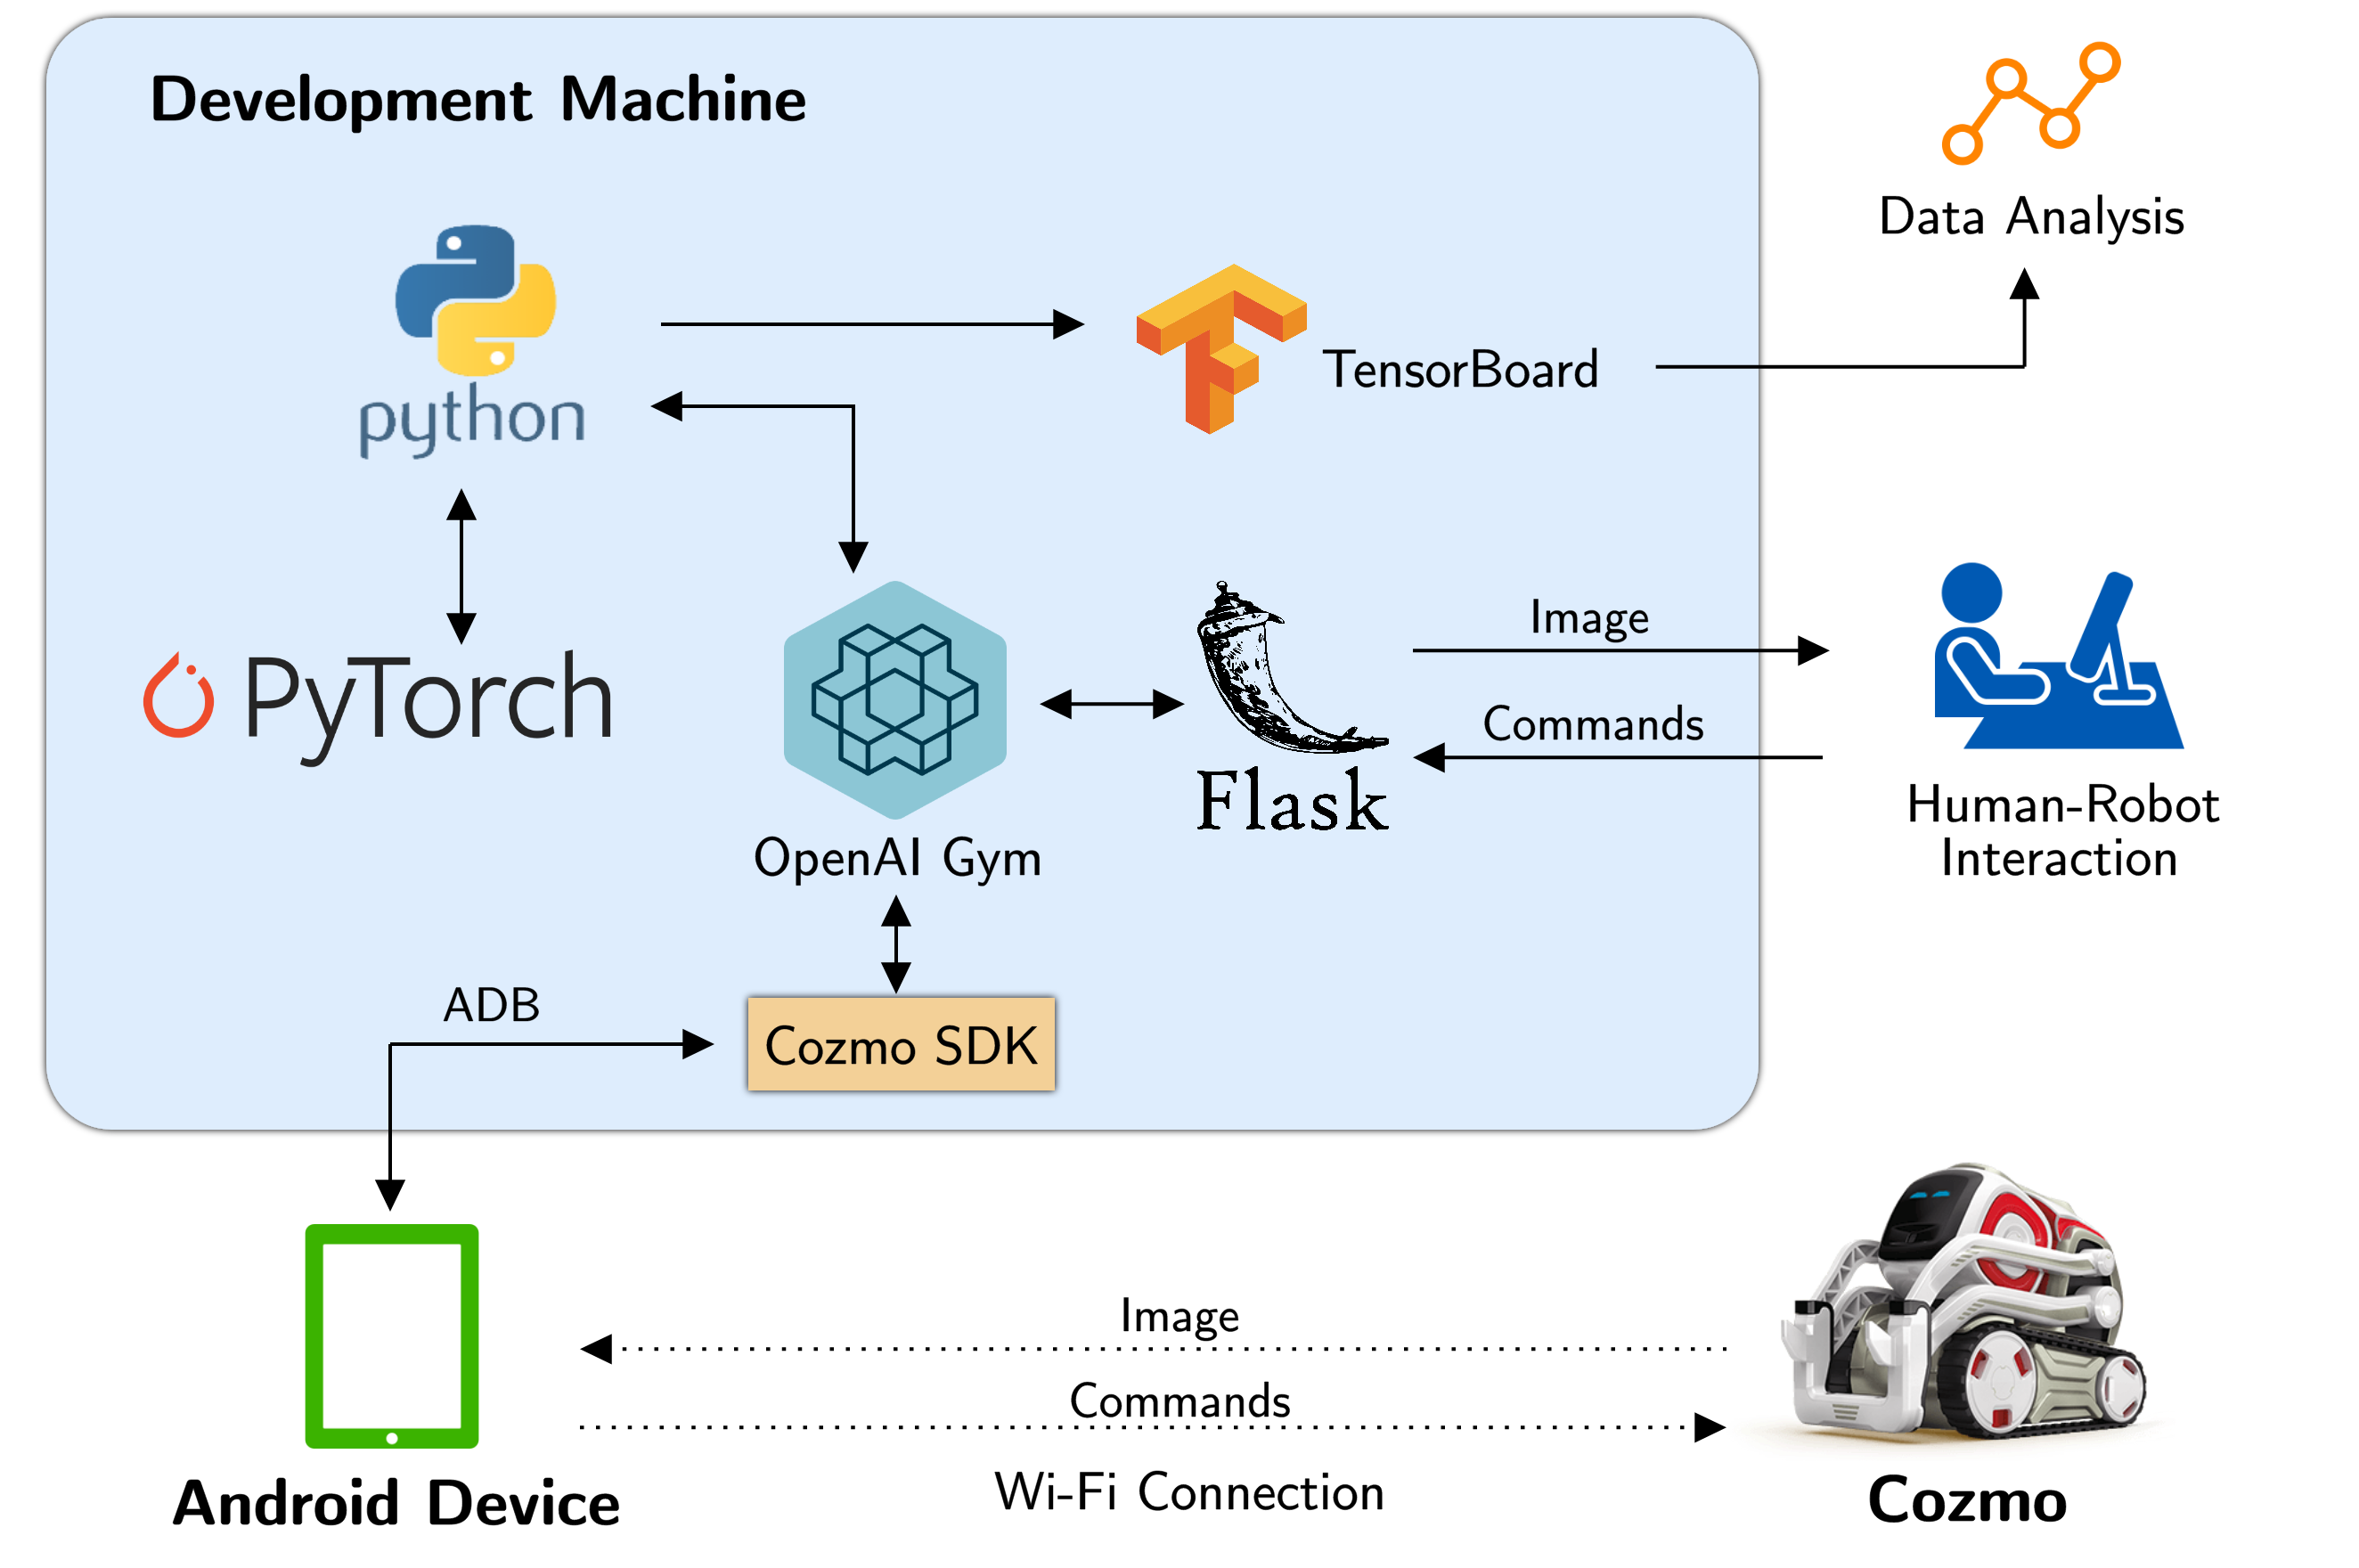
\includegraphics[width=0.97\columnwidth]{cozmo-system.png}
    \caption[Outline of the control system]{Outline of the control system that shows the most crucial technologies and component involved.}
    \label{system}
\end{figure}

To obtain this configuration, we managed to design a simple and intuitive user interface that prompt the user when he started an experiment. This interface provides a live stream from Cozmo on-board camera and a set of key with the related function. It works through Javascript to communicate to a Flask server that communicates directly to Cozmo SDK and the OpenAI Gym environment we designed to provide information for the user (e.g.\ images, learning information) and the robot (e.g.\ commands). The system we obtained is outlined in figure \ref{system}.

TODO:
\begin{itemize}
    \item MDP formalisation
\end{itemize}

\section{Experiments}

TODO:
\begin{itemize}
    \item Experiment Setup
    \item Cite preliminary experiment
    \item Showcase and comment about results with Cozmo Driver
\end{itemize}

\subsection{Experiments with Pendulum-v0}

\subsection{Experiments with CozmoDriver-v0}

\section{Conclusions}

TODO:
\begin{itemize}
    \item Conclusion
    \item Future Work
\end{itemize}

\subsection{Future Work}


{\small
    \bibliographystyle{ieee_fullname}
    \bibliography{egbib}
}

\end{document}
